\section{Betrachtung des Gesamtsystems}
% Gehäuse
% Stromverbrauch
\subsection{Software-Architektur}
Die Software lässt sich in zwei Einheiten unterteilen:
\begin{itemize}
  \item zeitkritische Operationen
  \item nichtzeitkritische Operationen
\end{itemize}
Zur Realisierung der zeitkritischen Operationen, wie dem Ticken der Uhr, dem Empfangen der Zeit sowie dem Ansteuern der LEDs wurden die Timer des AVR Mikrocontrollers benutzt. Der verwendetete ATmega32 besitzt drei Timer, einen 16-Bit- und zwei 8-Bit-Timer.

Die Timer senden in definierten Abständen Interrupts, die zur sofortigen Unterbrechung des Hauptprogrammes führen und den angegebenen Interrupt-Handler ausführen. Dazu wird der momentane Programmkontext auf den Stack gesichert, der Kontext für die Interrupt-Routine geladen, selbige ausgeführt und abschließend der Programmkontext wiederhergestellt, sodass die Ausführung des Programmes an der selben Stelle fortgeführt wird, wo es unterbrochen wurde. Unterbrechbar sind alle nicht-zeitkritischen Funktionen, die in der Endlosschleife der \texttt{main}-Methode des Programmes ausgeführt werden.

Der Programmablaufplan \ref{fig_pap} beschreibt die \texttt{main}-Methode sowie die drei Interrupt-Service-Routinen. In den folgenden Unterkapiteln werden die einzelnen Routinen nochmals textuell erläutert.
\begin{figure}[htp]
\centering
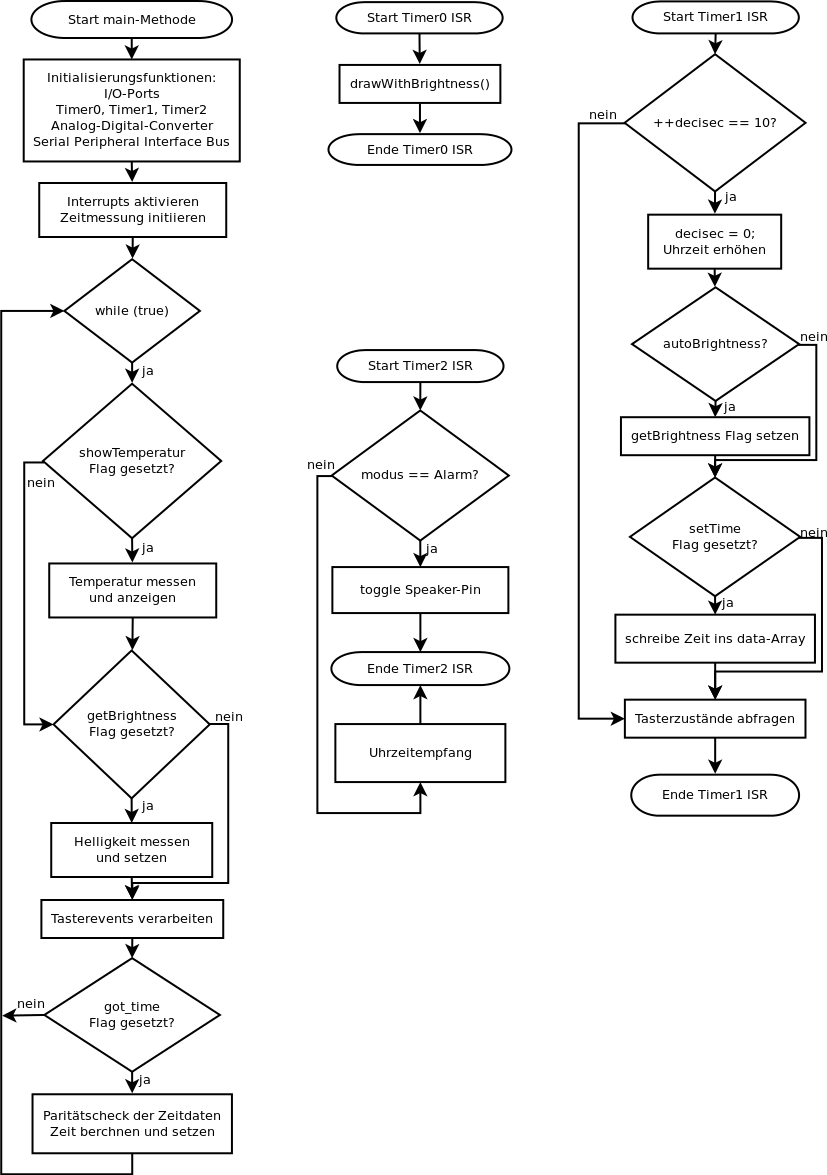
\includegraphics[width=\textwidth]{skizzen/papTimerAndMain.png}
\caption{Programmablaufplan für die main-Methode sowie die drei ISR}\label{fig_pap}
\end{figure}
%
\subsubsection{Ansteuern der LEDs - Timer0}\label{led_timer}
Zum Ansteuern der LEDs wurde der 8-Bit Timer0 im \glqq Interrupt by Overflow\grqq -Modus verwendet. Dies bedeutet, dass er bei jedem Überlauf, also von $2^8-1$ auf $0$, einen Interrupt erzeugt. In dem Setup wurde ein 14,7456 MHz Quarz sowie ein Prescaler von 8 verwendet. Dies sorgt dafür, dass nur in jedem 8. Taktschritt der Zähler des Timers inkrementiert wird. Daraus resultiert eine Interruptrate von $\frac{Clock}{Prescaler * Steps} = \frac{14745600 Hz}{8 * 2^8} = 7200 Hz$. Dies bedeutet, dass die Funktion \texttt{static inline void drawWithBrightness(void)} 7200 mal in der Sekunde aufgerufen wird. Diese Funktion steuert bei jedem Aufruf eine Reihe von LEDs an und inkrementiert den Reihenzähler anschließend. Es entsteht also bei 7 Aufrufen der Funktion ein gesamtes Bild und damit ist die Bildfrequenz $\frac{7200 Hz}{7} \approx 1028,57 Hz$. Dies wirkt zunächst viel, wird aber durch die Pulsweitenmodulation (siehe Kapitel \ref{sec_pulsweitenmodulation}) für die Helligkeitsabstufungen noch deutlich herabgesetzt.

\subsubsection{Ticken der Uhrzeit - Timer1}
Für die zeitlich kritischste Funktion, dem exakten Ticken der Uhrzeit wurde der 16-Bit Timer1 im \glqq CTC\grqq -Modus verwendet. CTC steht für Clear Timer on Compare Match und ist ein Modus, bei dem ein Höchstwert spezifiziert werden kann, bei dem der Timer einen Interrupt auslöst und sofort wieder bei 0 zu zählen beginnt. Damit kann ein taktgenauer Timer realisiert werden, wodurch kaum Abweichungen in der Uhrzeit entstehen.

Es wurde sich dafür entschieden, als kleinste Zeiteinheit Dezisekunden zu verwenden. Zur Anzeige der Uhrzeit ist dies allemal ausreichend, aber so kann dieser Timer zusätzlich dazu verwendet werden, die Tasterzustände abzufragen und wäre für eine etwaige Anwendung, wo Dezisekunden benötigt werden (bspw. Stoppuhr) vorbereitet.

Um den Timer also 10 mal pro Sekunde einen Interrupt erzeugen zu lassen, muss der Vergleichswert folgendermaßen gesetzt werden: $CMP = \frac{Takt}{\frac{INT}{s}} = \frac{14745600 Hz}{10 \frac{1}{s}} = 1474560$. Dieser Wert kann von einem 16-Bit Timer nicht erreicht werden, da $2^{16} < 1474560$. Deshalb muss auch hier ein Prescaler verwendet werden. Bei einem Prescaler von 1024 ergibt sich ein Wert von $\frac{1474560}{1024} = 1440$, welcher ideal ist, weil er einerseits innerhalb der 16-Bit Grenzen liegt und andererseits eine Ganzzahl ist, sodass genau bei jedem Interrupt eine Zehntelsekunde verstrichen ist.

Innerhalb der Timer1 Interruptroutine werden folgende Operationen ausgeführt:
\begin{enumerate}
  \item Die Uhrzeitvariablen (decisec, sec, min, hour) erhöhen
  \item Flag zum Messen der Helligkeit setzen
  \item Die Zeit neu in das Array zum Zeichnen schreiben
  \item Die Zustände der Taster abfragen
\end{enumerate}
 
\subsubsection{Empfangen der Uhrzeit - Timer2}
Der dritte Timer wird primär zum Empfangen der Uhrzeit verwendet, wird aber zusätzlich auch zur Tongenerierung für den Lautsprecher benutzt, wenn ein Alarm aktiv ist.

Auch dieser Timer wird im CTC-Modus verwendet, der Vergleichswert aber je nach Anwendung geändert. Beim Empfangen der Uhrzeit ist die Auflösung 10 ms und damit der $Vergleichswert = \frac{Takt}{Prescaler * \frac{INT}{s}} = \frac{14745600 Hz}{1024 * 100 \frac{1}{s}} = 144$. Innerhalb der Interruptroutine werden nun statusabhängige Funktionen zum Empfangen der Uhrzeit aufgerufen. Eine genauere Betrachtung dieser Funktionen ist in Kapitel \ref{sec_dcf77modul} zu finden.

Bei der Alarmfunktion wird der Wert abhängig der gewünschten Tonhöhe gesetzt.

\subsubsection{Nichtzeitkritische Funktionen in der main-Methode}
Alle Funktionen, bei denen die strikte zeitliche Einhaltung nicht wichtig ist, sind in der Hauptschleife des Programmes, einer \texttt{while(1)}-Schleife in der \texttt{main}-Methode zu finden.

Dort werden das Messen der Temperatur, sowie der Helligkeit vorgenommen. Außerdem werden dort Events behandelt, die beim Drücken der Taster auftreten sollen, wie das manuelle Umstellen der Zeit oder der Helligkeit und zu guter Letzt die Verifizierung und Konvertierung der in Interruptroutine von Timer2 empfangenen Uhrzeit. Zusammenfassend also alles Funktionen, die für den Betrieb der Digitaluhr wichtig sind, bei denen es aber nicht darauf ankommt, wann genau sie aufgerufen werden, sondern nur, dass sie aufgerufen werden. 

\subsection{Hardware}
\subsubsection{Hauptplatine}
Das Herzstück der Uhr ist die nachfolgend abgebildete Hauptplatine. Sie enthält den Mikrocontroller, einige wichtige Komponenten sowie die Anschlüsse für alle externen Komponenten. Unter der Abbildung sind die verwendeten Bauteile kurz beschrieben.

\begin{center}
\includegraphics[width=\textwidth]{images/platine.png}
\captionof{figure}{Hauptplatine der Digitaluhr}\label{img_platine}
\end{center}

\begin{list}{\ding{42}}
{\setlength{\topsep}{0cm}
\setlength{\itemsep}{0cm}
\setlength{\leftmargin}{3cm}
\setlength{\labelwidth}{3cm}
\setlength{\labelsep}{0cm}
\renewcommand{\makelabel}[1]{\textbf{\textsf{\normalsize #1} }}}
\item[1. Mikrocontroller ATmega32] Zentrale Steuereinheit\footnote{Pinbelegung des ATmega32 siehe Abbildung \ref{fig_belegung}}
\item[2. Mosfet IRF5305] zum Ansteuern der Kathoden der LED-Matrix
\item[3. Schieberegister TPIC6B595] zum Ansteuern der Anoden der LED-Matrix 
\item[4. 14,7456 MHz Quarz] als Taktgeber für den Mikrocontroller
\item[5. Potentiometer] für die Lautstärkeeinstellung der Weckfunktion
\item[6. Anschluss DCF77-Empfänger] für den Zeitempfang
\item[7. interne Taster] für verschiedene Einstellungsmöglichkeiten (bspw. Helligkeit)
\item[8. Anschluss für externe Taster] mit gleicher Belegung wie interne Taster
\item[9. Lagesensor] zum Erkennen, wie die Uhr aufgehängt ist
\item[10. ISP Schnittstelle] In-system programming zum Programmieren des Mikrocontrollers
\item[11. Anschluss Temperatursensor DS18S20] 
\item[12. Anschluss Fotowiderstand] zum Messen der Helligkeit
\item[13. Anschluss Stromquelle] für 5 Volt Gleichspannungsversorgung
\item[14. Resettaster] für den vollständigen Reset des Mikrocontrollers
\end{list}

\begin{center}
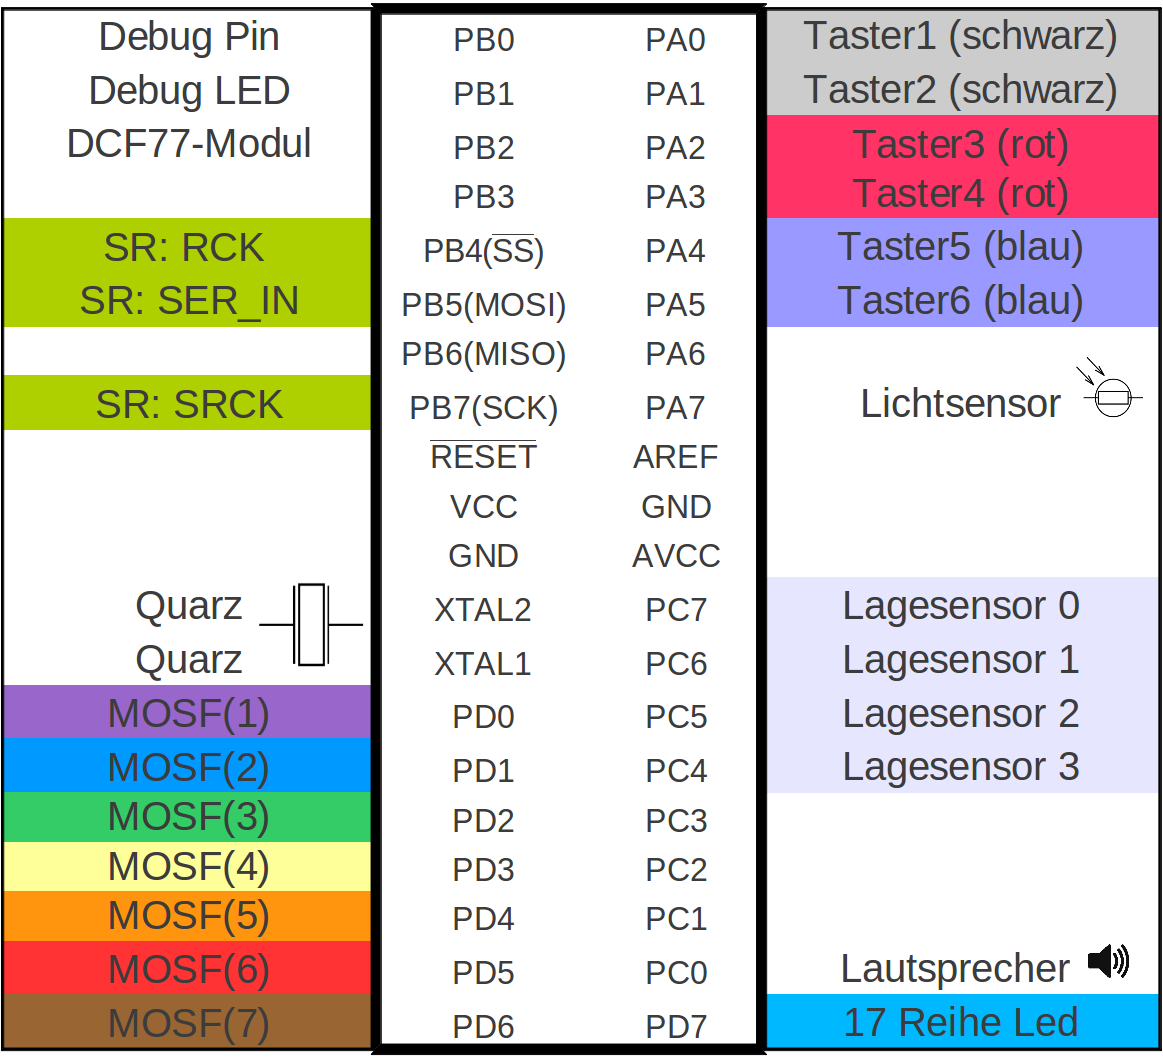
\includegraphics[width=.75\textwidth]{skizzen/AVR_Pinbelegung.png}
\captionof{figure}{Pinbelegung des ATmega32}\label{fig_belegung}
\end{center}
%\end{figure}

\subsubsection{Energieversorgung und Verbrauch}
Als Netzteil wurde ein CE geprüftes 5V/2A Netzteil gewählt. Das kompakte verwendete Schaltnetzteil ist ausreichend dimensioniert um den, mit einem Labornetzteil, ermittelten maximalen Bedarf von ca. 1.8A (alle LEDs aktiv bei maximaler Helligkeit) bereitzustellen.
 
Als Stromkabel kommt ein zweipoliges Kabel mit Schalter zum Einsatz. Dieses wurde im Inneren des Gehäuses mit Schmelzklebestoff verklebt und in eine Lüsterklemme geführt, so dass bei eventuell auftretenden Zugkräften auf keinen Fall Kräfte auf das Netzteil wirken.

Mittels des Temperatursensors wurde außerdem in einem Testlauf sichergestellt, dass die Temperatur im Inneren der Uhr 50\degree C (bei einer Raumtemperatur von 22\degree C) nicht überschreitet.
%
%
%
%eof
